\definecolor{Purple}{RGB}{120,28,129}
\definecolor{Blue}{RGB}{63,96,174}
\definecolor{Duck}{RGB}{83,158,182}
\definecolor{Green}{RGB}{109,179,136}
\definecolor{Yellow}{RGB}{202,184,67}
\definecolor{Orange}{RGB}{231,133,50}
\definecolor{Red}{RGB}{217,33,32}
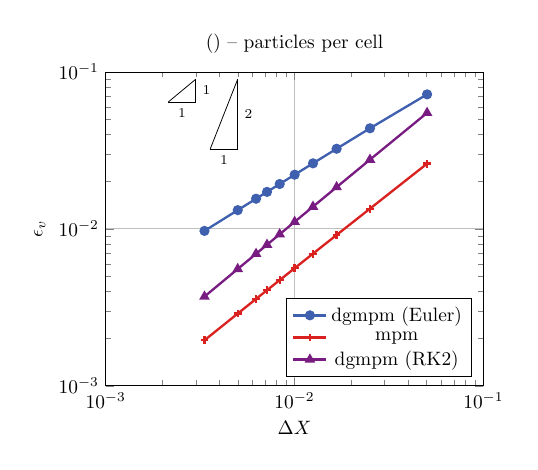
\begin{tikzpicture}[scale=0.7]
\begin{loglogaxis}[xlabel=$\Delta X$,ylabel=$\epsilon_v$,ymajorgrids=true,xmajorgrids=true,legend pos=south east,title={() -- particles per cell},xmin=0.001,xmax=0.1,ymin=0.001,ymax=0.1]
\addplot[Blue,very thick,mark=*] coordinates {(0.05031446540880504,0.07199248636963265) (0.025078369905956112,0.04376032394620455) (0.016701461377870562,0.0324206903335579) (0.01251956181533646,0.026165740820692437) (0.010012515644555693,0.022146057198539026) (0.008342022940563087,0.0193197079992959) (0.0071492403932082215,0.01721095122239602) (0.006254886630179829,0.015569904064014213) (0.0050031269543464665,0.013167396186349236) (0.003334722801167153,0.009707478832400305) };
\addplot[Red,very thick,mark=+] coordinates {(0.05031446540880504,0.026044883909926764) (0.025078369905956112,0.01345132435186097) (0.016701461377870562,0.009146551416522557) (0.01251956181533646,0.0069520075311606975) (0.010012515644555693,0.00561651057366531) (0.008342022940563087,0.004716438652201631) (0.0071492403932082215,0.004067898241443166) (0.006254886630179829,0.0035779713990584977) (0.0050031269543464665,0.0028862476375806695) (0.003334722801167153,0.0019511058389242168) };
\addplot[Purple,very thick,mark=triangle*] coordinates {(0.05031446540880504,0.05487193722857531) (0.025078369905956112,0.027617366247470396) (0.016701461377870562,0.0184516607190699) (0.01251956181533646,0.01385374680420358) (0.010012515644555693,0.01109019058982876) (0.008342022940563087,0.00924581913269737) (0.0071492403932082215,0.007927431853994336) (0.006254886630179829,0.00693810626040479) (0.0050031269543464665,0.005552280226022317) (0.003334722801167153,0.0037031152067471904) };
\legend{dgmpm (Euler),mpm,dgmpm (RK2)}
\draw (axis cs:0.003,0.09) -- (axis cs:0.003/1.4,0.09/1.4);
\draw (axis cs:0.003,0.09) -- (axis cs:0.003,0.09/1.4) node [midway,right] {\scriptsize 1};
\draw (axis cs:0.003,0.09/1.4) -- (axis cs:0.003/1.4,0.09/1.4) node [midway,below] {\scriptsize 1};
\draw (axis cs:0.005,0.09) -- (axis cs:0.005/1.4,0.09/2.8);
\draw (axis cs:0.005,0.09) -- (axis cs:0.005,0.09/2.8) node [midway,right] {\scriptsize 2};
\draw (axis cs:0.005,0.09/2.8) -- (axis cs:0.005/1.4,0.09/2.8) node [midway,below] {\scriptsize 1};
\end{loglogaxis}
\end{tikzpicture}
